\section{Gain saturation}

Gain saturation is a phenomenon that occurs when an amplifier device, such as a laser gain medium, cannot maintain a fixed gain for arbitrarily high input powers. This would require adding arbitrary amounts of power to the amplified signal.

For example, a sudden increase in the signal input power of a laser gain medium will reduce the gain only within a certain time because the population in excited laser ions is only reduced with a certain finite rate. This has important consequences for laser dynamics2.

In the steady state (i.e., for long time scales with constant pump power and resonator losses), the gain is where Psat is the saturation power. Note that it has been implicitly assumed that the pump rate is constant, i.e., there are no effects of pump saturation2.

The dynamic behavior of a laser is determined by the interaction of the intracavity light field with the gain medium. Essentially, the intracavity laser power can grow or decay exponentially according to the difference between gain and resonator losses, whereas the rate of change in the gain is determined by stimulated and spontaneous emission (and possibly by other effects such as quenching and energy transfer)3.

In the case of a laser gain medium, the gain does not instantly adjust to the level according to the optical input power because the gain medium stores some amount of energy (excitation energy of the laser-active ions, atoms or molecules), and the stored energy determines the gain. For example, a sudden increase in the signal input power of a laser gain medium will reduce the gain only within a certain time because the population in excited laser ions is only reduced with a certain finite rate. This has important consequences for laser dynamics2.

Gain saturation is a phenomenon that occurs when an amplifier device, such as a laser gain medium, cannot maintain a fixed gain for arbitrarily high input powers. This would require adding arbitrary amounts of power to the amplified signal. Therefore, the gain must be reduced for high input powers; this phenomenon is called gain saturation (or gain compression).

In the case of a laser gain medium, the gain does not instantly adjust to the level according to the optical input power because the gain medium stores some amount of energy (excitation energy of the laser-active ions, atoms or molecules), and the stored energy determines the gain. For example, a sudden increase in the signal input power of a laser gain medium will reduce the gain only within a certain time because the population in excited laser ions is only reduced with a certain finite rate. This has important consequences for laser dynamics.

\begin{figure}[h]
    \centering
    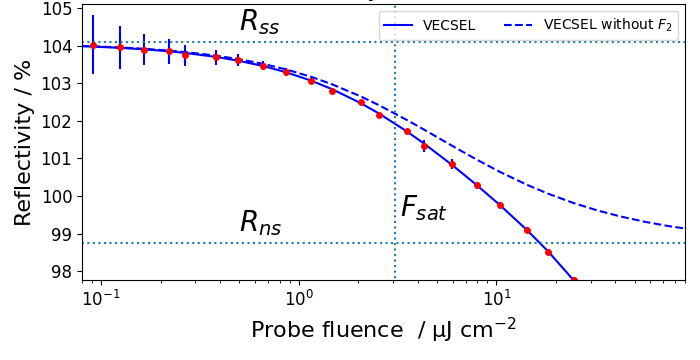
\includegraphics[width=12cm]{images/gainSat.png}
    \caption{}
\end{figure}